\documentclass[CJK]{beamer}
\usepackage{CJKutf8}
\usepackage{beamerthemesplit}
\usetheme{Malmoe}
\useoutertheme[footline=authortitle]{miniframes}
\usepackage{amsmath}
\usepackage{amssymb}
\usepackage{graphicx}
\usepackage{eufrak}
\usepackage{color}
\usepackage{slashed}
\usepackage{simplewick}
\usepackage{tikz}
\usepackage{ulem}
\usepackage{tcolorbox}
\graphicspath{{../figures/}}
%%figures
\def\lfig#1#2{\includegraphics[width=#1 in]{#2}}
\def\addfig#1#2{\begin{center}\includegraphics[width=#1 in]{#2}\end{center}}
\def\wulian{
\includegraphics[width=0.18in]{emoji_wulian.jpg}}
\def\bigwulian{
\includegraphics[width=0.35in]{emoji_wulian.jpg}}
\def\bye{
\includegraphics[width=0.18in]{emoji_bye.jpg}}
\def\bigbye{
\includegraphics[width=0.35in]{emoji_bye.jpg}}
\def\huaixiao{
\includegraphics[width=0.18in]{emoji_huaixiao.jpg}}
\def\bighuaixiao{
\includegraphics[width=0.35in]{emoji_huaixiao.jpg}}
\def\jianxiao{
\includegraphics[width=0.18in]{emoji_jianxiao.jpg}}
\def\bigjianxiao{
\includegraphics[width=0.35in]{emoji_jianxiao.jpg}}
%% colors
\def\blacktext#1{{\color{black}#1}}
\def\bluetext#1{{\color{blue}#1}}
\def\redtext#1{{\color{red}#1}}
\def\darkbluetext#1{{\color[rgb]{0,0.2,0.6}#1}}
\def\skybluetext#1{{\color[rgb]{0.2,0.7,1.}#1}}
\def\cyantext#1{{\color[rgb]{0.,0.5,0.5}#1}}
\def\greentext#1{{\color[rgb]{0,0.7,0.1}#1}}
\def\darkgray{\color[rgb]{0.2,0.2,0.2}}
\def\lightgray{\color[rgb]{0.6,0.6,0.6}}
\def\gray{\color[rgb]{0.4,0.4,0.4}}
\def\blue{\color{blue}}
\def\red{\color{red}}
\def\green{\color{green}}
\def\darkgreen{\color[rgb]{0,0.4,0.1}}
\def\darkblue{\color[rgb]{0,0.2,0.6}}
\def\skyblue{\color[rgb]{0.2,0.7,1.}}
%%control
\def\be{\begin{equation}}
\def\ee{\nonumber\end{equation}}
\def\bea{\begin{eqnarray}}
\def\eea{\nonumber\end{eqnarray}}
\def\bch{\begin{CJK}{UTF8}{gbsn}}
\def\ech{\end{CJK}}
\def\bitem{\begin{itemize}}
\def\eitem{\end{itemize}}
\def\bcenter{\begin{center}}
\def\ecenter{\end{center}}
\def\bex{\begin{minipage}{0.2\textwidth}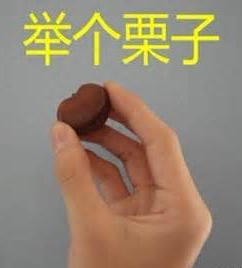
\includegraphics[width=0.6in]{jugelizi.png}\end{minipage}\begin{minipage}{0.76\textwidth}}
\def\eex{\end{minipage}}
\def\chtitle#1{\frametitle{\bch#1\ech}}
\def\bmat#1{\left(\begin{array}{#1}}
\def\emat{\end{array}\right)}
\def\bcase#1{\left\{\begin{array}{#1}}
\def\ecase{\end{array}\right.}
\def\bmini#1{\begin{minipage}{#1\textwidth}}
\def\emini{\end{minipage}}
\def\tbox#1{\begin{tcolorbox}#1\end{tcolorbox}}
\def\pfrac#1#2#3{\left(\frac{\partial #1}{\partial #2}\right)_{#3}}
%%symbols
\def\sone{$\star$}
\def\stwo{$\star\star$}
\def\sthree{$\star\star\star$}
\def\sfour{$\star\star\star\star$}
\def\sfive{$\star\star\star\star\star$}
\def\rint{{\int_\leftrightarrow}}
\def\roint{{\oint_\leftrightarrow}}
\def\stdHf{{\textit{\r H}_f}}
\def\deltaH{{\Delta \textit{\r H}}}
\def\ii{{\dot{\imath}}}
\def\skipline{{\vskip0.1in}}
\def\skiplines{{\vskip0.2in}}
\def\lagr{{\mathcal{L}}}
\def\hamil{{\mathcal{H}}}
\def\vecv{{\mathbf{v}}}
\def\vecx{{\mathbf{x}}}
\def\vecy{{\mathbf{y}}}
\def\veck{{\mathbf{k}}}
\def\vecp{{\mathbf{p}}}
\def\vecn{{\mathbf{n}}}
\def\vecA{{\mathbf{A}}}
\def\vecP{{\mathbf{P}}}
\def\vecsigma{{\mathbf{\sigma}}}
\def\hatJn{{\hat{J_\vecn}}}
\def\hatJx{{\hat{J_x}}}
\def\hatJy{{\hat{J_y}}}
\def\hatJz{{\hat{J_z}}}
\def\hatj#1{\hat{J_{#1}}}
\def\hatphi{{\hat{\phi}}}
\def\hatq{{\hat{q}}}
\def\hatpi{{\hat{\pi}}}
\def\vel{\upsilon}
\def\Dint{{\mathcal{D}}}
\def\adag{{\hat{a}^\dagger}}
\def\bdag{{\hat{b}^\dagger}}
\def\cdag{{\hat{c}^\dagger}}
\def\ddag{{\hat{d}^\dagger}}
\def\hata{{\hat{a}}}
\def\hatb{{\hat{b}}}
\def\hatc{{\hat{c}}}
\def\hatd{{\hat{d}}}
\def\hatN{{\hat{N}}}
\def\hatH{{\hat{H}}}
\def\hatp{{\hat{p}}}
\def\Fup{{F^{\mu\nu}}}
\def\Fdown{{F_{\mu\nu}}}
\def\newl{\nonumber \\}
\def\vece{\mathrm{e}}
\def\calM{{\mathcal{M}}}
\def\calT{{\mathcal{T}}}
\def\calR{{\mathcal{R}}}
\def\barpsi{\bar{\psi}}
\def\baru{\bar{u}}
\def\barv{\bar{\upsilon}}
\def\qeq{\stackrel{?}{=}}
\def\torder#1{\mathcal{T}\left(#1\right)}
\def\rorder#1{\mathcal{R}\left(#1\right)}
\def\contr#1#2{\contraction{}{#1}{}{#2}#1#2}
\def\trof#1{\mathrm{Tr}\left(#1\right)}
\def\trace{\mathrm{Tr}}
\def\comm#1{\ \ \ \left(\mathrm{used}\ #1\right)}
\def\tcomm#1{\ \ \ (\text{#1})}
\def\slp{\slashed{p}}
\def\slk{\slashed{k}}
\def\calp{{\mathfrak{p}}}
\def\veccalp{\mathbf{\mathfrak{p}}}
\def\Tthree{T_{\tiny \textcircled{3}}}
\def\pthree{p_{\tiny \textcircled{3}}}
\def\dbar{{\,\mathchar'26\mkern-12mu d}}
\def\erf{\mathrm{erf}}
\def\const{\mathrm{constant}}
\def\pheat{\pfrac p{\ln T}V}
\def\vheat{\pfrac V{\ln T}p}
%%units
\def\fdeg{{^\circ \mathrm{F}}}
\def\cdeg{^\circ \mathrm{C}}
\def\atm{\,\mathrm{atm}}
\def\angstrom{\,\text{\AA}}
\def\SIL{\,\mathrm{L}}
\def\SIkm{\,\mathrm{km}}
\def\SIyr{\,\mathrm{yr}}
\def\SIGyr{\,\mathrm{Gyr}}
\def\SIV{\,\mathrm{V}}
\def\SImV{\,\mathrm{mV}}
\def\SIeV{\,\mathrm{eV}}
\def\SIkeV{\,\mathrm{keV}}
\def\SIMeV{\,\mathrm{MeV}}
\def\SIGeV{\,\mathrm{GeV}}
\def\SIcal{\,\mathrm{cal}}
\def\SIkcal{\,\mathrm{kcal}}
\def\SImol{\,\mathrm{mol}}
\def\SIN{\,\mathrm{N}}
\def\SIHz{\,\mathrm{Hz}}
\def\SIm{\,\mathrm{m}}
\def\SIcm{\,\mathrm{cm}}
\def\SIfm{\,\mathrm{fm}}
\def\SImm{\,\mathrm{mm}}
\def\SInm{\,\mathrm{nm}}
\def\SImum{\,\mathrm{\mu m}}
\def\SIJ{\,\mathrm{J}}
\def\SIW{\,\mathrm{W}}
\def\SIkJ{\,\mathrm{kJ}}
\def\SIs{\,\mathrm{s}}
\def\SIkg{\,\mathrm{kg}}
\def\SIg{\,\mathrm{g}}
\def\SIK{\,\mathrm{K}}
\def\SImmHg{\,\mathrm{mmHg}}
\def\SIPa{\,\mathrm{Pa}}

\title{Dark Energy}
\author{Zhiqi Huang}
\institute{Sun Yat-sen University}
\date{June 12, 2017}


\begin{document}

\begin{frame}
  \bcenter
      {\Huge Dark Energy}

      \addfig{2.2}{Dark_Energy.jpg}
      
      Zhiqi Huang


      {\small School of Physics and Astronomy, Sun Yat-sen University}
      
      {\small April 4th, 2018}
      
      \ecenter
\end{frame}

\begin{frame}
\frametitle{Why the slides are in English}
           {\Large
             Every time I gave a lecture, the students wrote (=Ctrl C + Ctrl V) awful term essays and asked me not to fail them.

}
\end{frame}


\begin{frame}
\chtitle{Fundamental Problems in Physics}
\centering
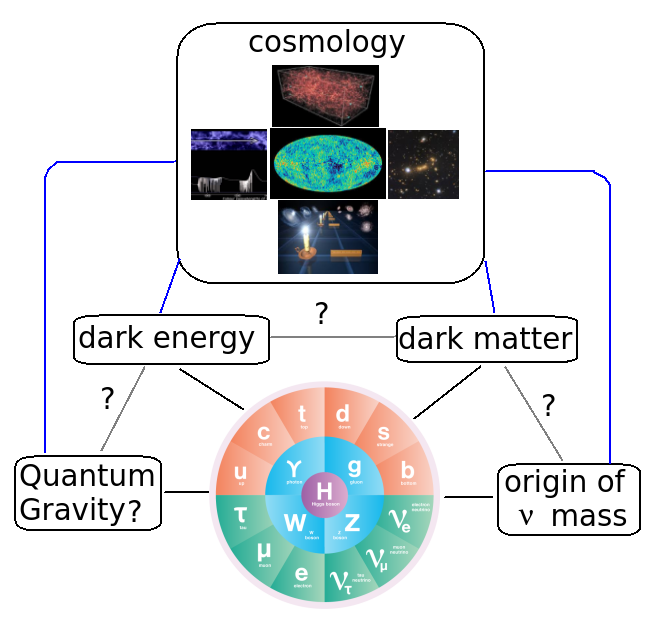
\includegraphics[width=3.in]{cosmo_value2.png}
\end{frame}


\begin{frame}
\frametitle{Outline}
\bitem
\item{The Dark Universe}
\item{Cosmic Acceleration and Dark Energy}
\item{The Nature of Dark Energy}
\eitem
\end{frame}


\section{The Dark Universe}

\begin{frame}
  \frametitle{Milky Way and Dark Matter Halo}
  \addfig{2.6}{DarkMilkyWay.jpg}
\end{frame}

\begin{frame}
  \frametitle{View on Large Scales}
  \addfig{3.4}{darkweb.jpg}
\end{frame}


\section{Cosmic Acceleration and Dark Energy}

\begin{frame}
  \frametitle{The Universe is Expanding}
  \addfig{3}{expanding-universe.jpg}

  Discovered by Edwin Hubble (no Nobel Prize).
\end{frame}


\begin{frame}
  \frametitle{Measuring the Distance: Standard Candles and Standard Rulers}

  \addfig{3.5}{distance_measure.jpg}


\end{frame}

\begin{frame}
  \frametitle{Measuring the Velocity: Doppler Effect}

  \addfig{3.5}{doppler.png}

(In Einstein's General Relativity, the ``velocity'' should be interpreted as expansion of space.)
\end{frame}



\begin{frame}
  \frametitle{Can be Explained by Bigbang}
  \addfig{3.5}{bigbang.jpg}
\end{frame}


\begin{frame}
  \frametitle{Friedmann Equation}
             {\Large

               Energy Conservation:
               
    $$ \left(\frac{\dot a}{a}\right)^2 = \frac{8\pi G}{3}\rho. $$

    }
\end{frame}


\begin{frame}
  \frametitle{Accelerated Expansion}
  \addfig{2}{Dark_Energy.jpg}
  
{\Large
  $$\ddot a > 0. $$
  (Nobel Prize)
  }
\end{frame}

\begin{frame}
  \frametitle{A big question}

  \addfig{1}{think2.jpg}
  {\Large

    If gravity is always attractive, how to accelerate the expansion?}
\end{frame}


\begin{frame}
  \frametitle{Cosmological Constant (Vacuum Energy)}
  General Relativity:  effective ``gravitational mass'' = $\rho + 3 p $

\lfig{2}{scales.jpg}\lfig{2}{scales2.jpg}
  
  \bitem
\item{nonrealivistic matter $p\ll \rho$ $\Rightarrow$  Newtonian gravity}
\item{Radiation $p = \frac{1}{3} \rho$ $\Rightarrow$ twice Newtonian gravity}
\item{vacuum energy $ p= -\rho$ $\Rightarrow$ repulsive force}
  \eitem

\end{frame}


\begin{frame}
  \frametitle{Puzzles}

  Cosmological Constant $\Lambda$
  
  \addfig{1}{blackq.jpg}

  \bitem
\item{Why so small? ($\sim 10^{-120}\times$ naive dimension analysis)}
\item{Why this small? ($\sim 2 \rho_{\rm matter}$)}
  \eitem
\end{frame}


\begin{frame}
  \frametitle{$H_0$ tension}
  Hubble Constant $H_0$: expansion rate of the Universe
  \skipline

  \addfig{2}{H0tension.pdf}
  
  Local (current)  measurement (Riess {\it et al}, 2018): $H_0 = 73.48\pm 1.66\, \mathrm {km\,s^{-1}Mpc^{-1}}$.

  \skipline
  
  Distant (early) measurement (Planck collaboration, 2016): $H_0 = 67.51\pm 0.64 \, \mathrm {km\,s^{-1}Mpc^{-1}}$.
\end{frame}

\begin{frame}
  \frametitle{Other Dark Energy Models}
  \begin{Large}
  \bitem
\item{quintessence}
\item{k-essence}
\item{$f(R)$ gravity}
\item{scalar-tensor theory}
\item{Chaplygin gas}  
\item{holographic dark energy}
\item{\ldots}
  \eitem
  \end{Large}
\end{frame}

\begin{frame}
  \frametitle{Do Other Models Help?}
  \begin{Large}
    So far as we know, all of them
    \bitem
  \item{are more complicated.}
  \item{do not answer ``why so small''.}
  \item{do not answer ``why this small''.}
  \item{do not resolve $H_0$ tension}
    \eitem
  \end{Large}
\end{frame}


\begin{frame}
  \frametitle{Quintessence + spatial curvature do not solve $H_0$ tension}
  \begin{Large}
    \lfig{2}{qkcdm_H0_1D.pdf} \lfig{2}{qkcdm_H0_wa_2D.pdf}

    Miao and Huang, 2018
  \end{Large}
\end{frame}


\begin{frame}
  \frametitle{Coffee Break Story: Equipartition Dark Energy}
  \addfig{4}{equide.png}
\end{frame}

\begin{frame}
  \frametitle{Answers ``why so small'' and ``why this small''}

In this article we propose a new interpretation for dark energy. In the string landscape picture, the Universe was 11-dimension before spontaneous symmetry breaking and a 3-dimensional inflation took place. During inflation, the size of our 3-dimensional space soon exponentially exceeded the other spatial dimensions. The extra spatial dimensions became invisible and remained so until the Universe became cool enough to allow energy to tunnel from extra dimensions, which we interpret as dark energy. When the quantum tunneling reaches an equilibrium, the dark energy fraction can be estimated with equipartition theorem as
\begin{equation}
  \Omega_{\rm DE} \approx \frac{10-3}{10} = 0.7, \label{eq:eq}
\end{equation}
\end{frame}


\begin{frame}
  \frametitle{Resolves $H_0$ Tension}
  
  \lfig{2}{H0.pdf}\lfig{2}{prob.pdf}

  The consequence of energy communication between our universe and extra dimensions is that the Hubble parameter is no longer determined by the total energy density. In this way, the locally measured $H_0$ decouples from CMB constraints.

\end{frame}


\begin{frame}
  \frametitle{Coffee Break Story: Equipartition Dark Energy}
\lfig{1.8}{wechat01.png} \lfig{1.8}{wechat02.png}
\end{frame}


\begin{frame}
  \frametitle{Coffee Break Story: Equipartition Dark Energy}
\addfig{2.5}{timeline0.png}
\end{frame}

\begin{frame}
  \frametitle{Coffee Break Story: Equipartition Dark Energy}
\addfig{2.5}{timeline1.png}
\end{frame}


\begin{frame}
  \frametitle{Coffee Break Story: Equipartition Dark Energy}
\addfig{3}{timeline2.png}
\end{frame}


\begin{frame}
  \frametitle{Citation Request}
  \addfig{4.5}{spam2.png}
\end{frame}


\begin{frame}
  \frametitle{Look Familiar...}
  \addfig{4.5}{spam1.png}
\end{frame}

\begin{frame}
  \addfig{4.5}{citereq.png}
\end{frame}


\begin{frame}

  \begin{center}
    
  {\Huge Merci Beaucoup!}

  \skiplines
  
  {\large I didn't say anything and you won't write anything.}
  \end{center}

\end{frame}



\end{document}



